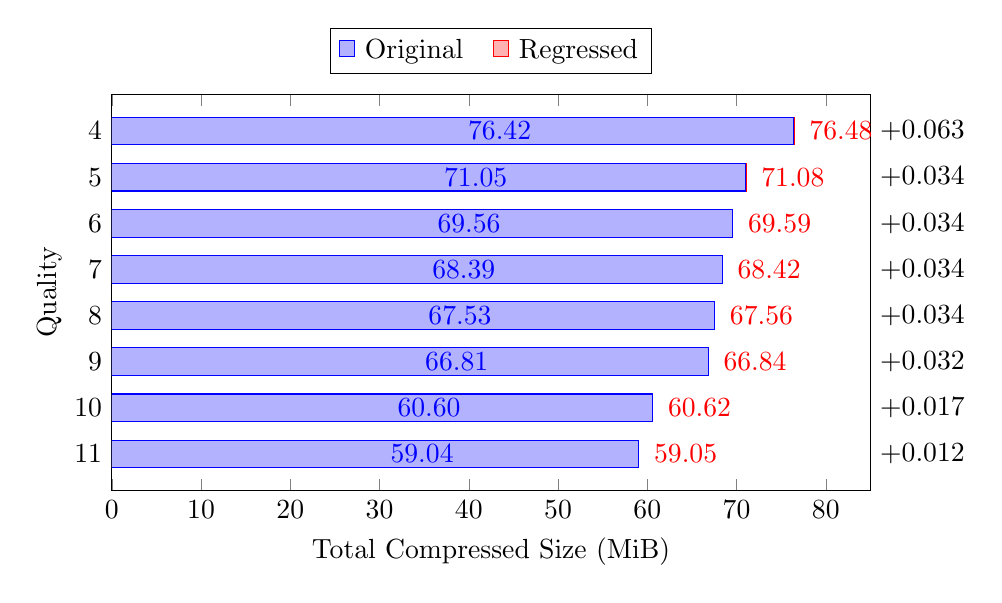
\begin{tikzpicture}
\begin{axis}[
	width = 0.925\textwidth,
	height = 0.91*\axisdefaultheight,
	xbar stacked,
	xmin = 0,
	xmax = 85,
	xtick distance = 10,
	y dir = reverse,
	ytick = data,
	ytick pos = left,
	extra y ticks = {4, 5, 6, 7, 8, 9, 10, 11},
	extra y tick labels = {$+0.063$, $+0.034$, $+0.034$, $+0.034$, $+0.034$, $+0.032$, $+0.017$, $+0.012$},
	extra y tick style = {ticklabel pos = right},
	scaled ticks = false,
	enlarge x limits = {abs = 0},
	enlarge y limits = {abs = 0.8},
	nodes near coords,
	nodes near coords align = {horizontal},
	nodes near coords style = {xshift = 2pt, /pgf/number format/.cd, fixed zerofill, precision = 2},
	legend columns = -1,
	legend style = {
		at = {(0.5, 1.05)},
		anchor = south,
		column sep = 0.05cm,
		/tikz/every even column/.append style = {
			column sep = 0.3cm
		}
	},
	legend image code/.code = {
		\draw[#1] (0cm, -0.075cm) rectangle (0.2cm, 0.135cm);
	},
	xlabel = Total Compressed Size (MiB),
	ylabel = Quality,
	ylabel style = {yshift = -width(+0.000)}
]
\legend{
	Original,
	Regressed
}
\addplot[blue, fill = blue!30!white] coordinates {
	(76.42, 4)
	(71.05, 5)
	(69.56, 6)
	(68.39, 7)
	(67.53, 8)
	(66.81, 9)
	(60.60, 10)
	(59.04, 11)
};
\addplot[red, fill = red!30!white, point meta = x] coordinates {
	(0.0634, 4)
	(0.0339, 5)
	(0.0343, 6)
	(0.0341, 7)
	(0.0340, 8)
	(0.0322, 9)
	(0.0172, 10)
	(0.0115, 11)
};
\end{axis}
\end{tikzpicture}